\cleardoublepage % memastikan bab baru dimulai di halaman ganjil (kanan)
\chapter{STUDI LITERATUR}
\label{chap:studi-literatur}

\section{Pengetahuan tentang Kasus yang Dikaji: Manajemen Informasi Gudang FMCG}

\subsection{Karakteristik Operasional Inventori Gudang FMCG Berbasis Pull System}
Pada industri \textit{Fast Moving Consumer Goods} (FMCG), gudang penyimpanan berperan sebagai pusat kendali aliran barang dalam rantai pasok yang menuntut kecepatan, akurasi, dan integrasi sistem yang tinggi. Operasional gudang yang efektif harus mampu menangani volume barang yang besar, variasi \textit{Stock Keeping Unit} (SKU) yang luas, serta kecepatan distribusi yang tinggi guna memastikan ketersediaan produk di pasar. Dalam konteks ini, gudang bukan lagi sekadar tempat penyimpanan pasif, melainkan komponen strategis yang secara langsung menentukan kelancaran seluruh rantai distribusi. \textcite{framinan2025} menegaskan bahwa sistem pergudangan konvensional pada industri FMCG mengandung inefisiensi signifikan akibat keterbatasan otomasi dan sistem informasi yang belum terintegrasi sepenuhnya, yang pada akhirnya berdampak pada keterlambatan pengiriman dan ketidakakuratan data inventori.

Secara operasional, terdapat empat sumber daya utama yang menggerakkan sebuah gudang, yaitu \textit{storage system}, \textit{lift trucks}, \textit{personnel}, dan \textit{Warehouse Management System} (WMS). Setiap komponen tersebut harus memenuhi \textit{Flow Impact Test} (IFIT), di mana kapasitas setiap komponen berpengaruh langsung terhadap kapasitas atau laju keseluruhan operasional gudang \autocite{brazhkin2018}. Keempat sumber daya ini bersifat saling bergantung dan harus beroperasi secara terkoordinasi untuk menjamin kelancaran alur barang dari tahap penerimaan hingga pengiriman akhir. Kegagalan pada salah satu komponen sumber daya akan menimbulkan efek domino yang mengganggu keseluruhan rantai operasional di dalam gudang.

Proses operasional inventori di dalam gudang secara umum mencakup sembilan tahapan utama, yaitu penerimaan (\textit{receiving}), penempatan (\textit{put-away}), pengisian ulang internal (\textit{internal replenishment}), pengambilan pesanan (\textit{order picking}), pengumpulan dan penyortiran (\textit{accumulating and sorting}), pengepakan (\textit{packing}), lintas-dermaga (\textit{cross docking}), pengiriman barang (\textit{dispatch}), dan pengapalan (\textit{shipping}) \autocite{habazin2017}. Di antara seluruh tahapan tersebut, proses \textit{order picking} menjadi titik paling kritis karena memiliki tingkat keterlibatan manual tertinggi dan paling rentan terhadap kesalahan serta keterlambatan. Studi empiris pada industri manufaktur di Kroasia menemukan bahwa kekurangan sumber daya manusia merupakan kendala dengan nilai keparahan rata-rata (\textit{mean severity}) kedua tertinggi dalam proses \textit{picking} di gudang dengan nilai 3,79 dari skala 5 \autocite{habazin2017}, yang mengindikasikan tingginya ketergantungan terhadap faktor manusia dalam aktivitas inti pergudangan konvensional.

\textcite{vangeest2021} menegaskan bahwa kompleksitas rantai pasok modern pada industri FMCG telah mendorong evolusi konsep gudang konvensional menuju \textit{Smart Warehouse}, yang dicirikan oleh empat pilar utama, yaitu \textit{Automation and Robotics}, \textit{IoT-based Visibility}, \textit{AI-driven Optimization}, dan \textit{Cyber-Physical Integration}. Dalam konteks operasional berbasis \textit{pull system}, pilar \textit{Cyber-Physical Integration} menjadi sangat krusial karena memungkinkan sinkronisasi antara permintaan digital dan eksekusi fisik berlangsung secara \textit{real-time}. Dengan demikian, setiap aktivitas pergerakan barang mulai dari penerimaan, penyimpanan, hingga pengiriman dapat tercatat dan direspons secara otomatis oleh sistem tanpa keterlambatan akibat keterbatasan proses manual.

\subsubsection*{Profil Sistem Operasional Gudang Paragon Corp Berdasarkan Hasil Wawancara}
Guna memperoleh gambaran kondisi operasional yang akurat dan kontekstual, kelompok TA252601001 melaksanakan wawancara daring dengan Bapak Falih Muhtadi selaku \textit{Staff Logistics and Business Integration Systems} PT Paragon Technology and Innovation (Paragon Corp) pada tanggal 16 Oktober 2025. Dari wawancara tersebut diketahui bahwa Paragon Corp memiliki tiga jenis gudang, yaitu gudang bahan baku, gudang kemasan (\textit{packaging warehouse}), serta gudang barang jadi (\textit{Finished Goods}) yang terletak pada area terpisah. Fokus pengembangan tugas akhir ini adalah pada gudang barang jadi, yang secara langsung bersinggungan dengan proses distribusi produk ke konsumen akhir.

Berdasarkan hasil wawancara, sistem kerja operasional inventori Paragon Corp menerapkan pendekatan \textit{Pull System}, yaitu suatu mekanisme di mana pergerakan dan pemrosesan barang didasarkan pada permintaan aktual yang masuk ke sistem, bukan pada prakiraan (\textit{forecasting}) internal. Alur kerja utama gudang mencakup empat tahapan, yaitu \textit{Incoming}, \textit{Stocking}, \textit{Picking \& Checking}, serta \textit{Dispatching} menuju \textit{Distribution Center}. Dalam skema \textit{pull system}, perintah \textit{stocking} dan \textit{picking} baru dieksekusi ketika terdapat permintaan nyata, sehingga meminimalkan akumulasi stok berlebih (\textit{overstock}) namun di sisi lain menuntut kecepatan respons sistem yang sangat tinggi agar tidak menimbulkan \textit{bottleneck} pada tahap distribusi.

Dari hasil wawancara juga terungkap bahwa teknologi yang saat ini digunakan di gudang Paragon mencakup sistem ERP Odoo dan \textit{Warehouse Management System} (WMS) untuk pencatatan dan pelacakan barang. Namun, kedua sistem tersebut masih bersifat semi-manual sehingga membutuhkan input operator secara berkala dan belum memiliki integrasi \textit{real-time} antar platform. Kondisi ini menyebabkan \textit{mismatch} data yang sering terjadi antara kondisi fisik di lapangan dengan catatan digital pada sistem pusat. Paragon Corp sendiri saat ini tengah dalam proses transformasi menuju sistem SAP untuk meningkatkan kualitas integrasi antar sistem. Kompleksitas operasional semakin bertambah mengingat Paragon Corp mengelola lebih dari 40 \textit{Distribution Centers} (DC) di Indonesia dan Malaysia \autocite{undip2019}, dengan volume produk dan variasi SKU kosmetik yang sangat beragam, sehingga ketersediaan sistem inventori yang akurat dan terintegrasi menjadi kebutuhan operasional yang mendesak.

\subsection{Identifikasi Masalah Sinkronisasi Data Stok}
Permasalahan inti yang menjadi landasan pengembangan \textit{Warehouse Management Controller} (WMC) dalam tugas akhir ini adalah ketidaksinkronan data stok antara kondisi fisik di lapangan dengan catatan digital pada sistem pusat, yang dikodekan sebagai Masalah Aktual pertama (MA01) dalam dokumen B100. Dalam kondisi eksisting, \textit{Warehouse Management System} (WMS) gudang barang jadi Paragon Corp beroperasi secara independen tanpa koneksi langsung ke sistem pusat perusahaan, sehingga pembaruan data stok masih bergantung pada intervensi manual operator. Akibatnya, terdapat jeda waktu yang tidak dapat diprediksi antara perubahan kondisi fisik barang di lapangan dengan refleksinya pada sistem informasi, sehingga data yang tersedia di sistem pusat tidak selalu mencerminkan kondisi aktual yang terjadi di gudang.

Ketidaksinkronan ini menghasilkan dua manifestasi utama yang secara langsung mengganggu efisiensi operasional. Pertama, terjadi \textit{mismatch} data stok, yaitu selisih antara jumlah barang yang tercatat di sistem dengan jumlah fisik yang tersedia di rak gudang. Kondisi ini memicu \textit{human error} pada proses \textit{picking}, terutama dalam konteks ketidaktepatan jumlah barang yang diambil, karena operator berpatokan pada data yang tidak akurat. Kedua, terjadi \textit{mistracking} barang, di mana posisi fisik barang tidak terdokumentasikan secara akurat karena terdapat area penempatan sementara yang tidak tercatat di dalam sistem manajemen gudang yang ada. Kedua masalah ini secara kumulatif menyebabkan \textit{bottleneck} pada tahap \textit{stocking} dan \textit{picking}, yang berujung pada kondisi \textit{overcapacity} serta \textit{waiting time} yang panjang di area gudang barang jadi.

Temuan ini sejalan dengan penelitian \textcite{framinan2025} yang mengkaji ulang proses pemenuhan pesanan pada perusahaan FMCG menggunakan metode \textit{Business Process Redesign} (BPR). Penelitian tersebut menemukan bahwa 62\% keterlambatan pengiriman bersumber dari aktivitas \textit{order picking} dan \textit{staging} yang tidak terkoordinasi secara digital, di mana sistem pencatatan yang tidak \textit{real-time} menjadi akar utama inefisiensi. Relevansi temuan ini terhadap kondisi Paragon Corp sangat tinggi, mengingat kedua sistem beroperasi dengan pola semi-manual yang serupa dalam konteks industri FMCG dengan volume tinggi dan variasi SKU yang luas.

\textcite{vangeest2021} mengidentifikasi interoperabilitas sistem sebagai salah satu tantangan teknologi paling kritis dalam implementasi \textit{Smart Warehouse}. Tantangan ini mencakup ketidakmampuan platform yang berbeda untuk saling bertukar data secara langsung, latensi sistem berbasis \textit{cloud}, dan potensi kehilangan data akibat ketidaksesuaian protokol komunikasi antar sistem. Dalam konteks gudang Paragon, kondisi tersebut tercermin dari ketidakterhubungan antara WMS lokal dengan sistem ERP Odoo, yang masing-masing beroperasi sebagai silo informasi yang berdiri sendiri tanpa mekanisme sinkronisasi otomatis.

Berdasarkan analisis \textit{gap} yang dilakukan pada dokumen B100, kondisi eksisting (MA01) ditargetkan untuk ditransformasi menjadi sistem yang sepenuhnya terintegrasi dan tersinkronisasi secara \textit{real-time} antara gudang barang jadi dan sistem pusat. Kebutuhan ini diformulasikan dalam dokumen B200 sebagai karakteristik fungsi dasar pertama sistem, yaitu CH01: sistem dapat menyinkronkan data stok secara otomatis antara kondisi fisik dan catatan digital untuk menjaga konsistensi informasi inventori. Dari sisi parameter kinerja, spesifikasi \textit{traceability} menetapkan bahwa sinkronisasi waktu antara robot dan server serta antara server dan WMS harus berada di bawah 200 milidetik, dengan pembaruan status robot ke server dilakukan dengan latensi tidak lebih dari 1 detik pada kondisi jaringan yang stabil \autocite{docB200}.

Oleh karena itu, perancangan \textit{Warehouse Management Controller} (WMC) sebagai layanan \textit{backend} dalam tugas akhir ini secara langsung merespons \textit{gap} sinkronisasi ini. WMC dirancang untuk menjadi titik kendali tunggal yang mencatat setiap aktivitas pergerakan barang sebagai sebuah \textit{event} digital, memastikan bahwa setiap tindakan fisik yang dilakukan oleh robot di lapangan secara otomatis memperbarui catatan stok pada basis data terpusat dan dapat diakses oleh sistem pusat tanpa memerlukan intervensi operator. Dengan demikian, pendekatan ini diharapkan dapat menutup \textit{gap} MA01 secara fundamental dan menjamin konsistensi data inventori secara menyeluruh di seluruh lapisan sistem.

\subsection{Konsep Digitalisasi Smart Warehouse}
Konsep digitalisasi \textit{Smart Warehouse} merupakan transformasi menyeluruh dari sistem pergudangan konvensional menuju sistem yang cerdas dan terhubung secara digital, dengan menempatkan data sebagai aset operasional utama. \textcite{vangeest2021} mendefinisikan \textit{Smart Warehouse} melalui empat pilar teknologi penggerak (\textit{technology enabler}), yaitu \textit{Automation and Robotics} untuk otomasi proses fisik, \textit{IoT-based Visibility} untuk deteksi dan pelacakan barang secara \textit{real-time}, \textit{AI-driven Optimization} untuk penjadwalan dan pengambilan keputusan otomatis, serta \textit{Cyber-Physical Integration} sebagai sinergi antara operasi fisik dan visibilitas data berbasis \textit{cloud}. Dalam perspektif sistem cerdas, \textcite{romero2020} menegaskan bahwa sebuah \textit{smart system} dicirikan oleh adanya elemen sistem, relasi antar entitas, objektif yang terukur, batasan lingkungan, dan antarmuka yang mengintegrasikan sistem dengan dunia luar. \textit{Smart Warehouse} memenuhi seluruh karakteristik tersebut dengan objektif tunggal: meningkatkan produktivitas dan akurasi operasional gudang secara berkelanjutan.

Dalam konteks tugas akhir ini, pilar \textit{Cyber-Physical Integration} menjadi landasan konseptual yang paling relevan bagi pengembangan \textit{Warehouse Management Controller} (WMC). Integrasi siber-fisik mengacu pada sinergi antara lapisan fisik---yaitu pergerakan robot dan barang di dalam gudang---dengan lapisan digital berupa pencatatan data inventori secara \textit{real-time} pada basis data terpusat berbasis \textit{cloud}. Melalui pendekatan ini, setiap aktivitas fisik di lapangan, mulai dari penerimaan barang (PA01), penyimpanan cerdas (PA02), hingga proses \textit{picking} dan manajemen gudang (PA03), secara otomatis tercermin dalam sistem informasi digital tanpa memerlukan intervensi manual. Digitalisasi berbasis \textit{Cyber-Physical Integration} inilah yang menjadi dasar arsitektur WMC, di mana setiap perintah robot dan setiap perubahan status barang diperlakukan sebagai \textit{event} yang langsung direkam dan disinkronkan ke seluruh lapisan sistem.

\section{Landasan Teori: Metode Perancangan dan Evaluasi Perangkat Lunak}

\subsection{Metode Analytical Hierarchy Process (AHP)}
\textit{Analytical Hierarchy Process} (AHP) adalah metode pengambilan keputusan multi-kriteria yang dikembangkan oleh Thomas L. Saaty pada tahun 1970-an. Metode ini bekerja dengan menyusun permasalahan keputusan ke dalam struktur hierarki yang terdiri dari tiga tingkat utama, yaitu tujuan (\textit{goal}), kriteria, dan alternatif solusi. Pada setiap tingkatan, AHP menggunakan teknik perbandingan berpasangan (\textit{pairwise comparison}) untuk mengukur tingkat kepentingan relatif antara satu elemen dengan elemen lainnya menggunakan skala numerik 1 hingga 9 yang dikembangkan oleh Saaty. Hasil perbandingan tersebut diolah melalui perhitungan bobot prioritas (\textit{eigenvector}) dan divalidasi melalui uji konsistensi dengan indikator \textit{Consistency Ratio} (CR), di mana nilai CR di bawah 0,1 mengindikasikan bahwa penilaian yang dilakukan bersifat konsisten dan dapat diterima \autocite{saaty1977}. Dalam konteks proyek \textit{Smart Warehouse} ini, metode AHP telah diimplementasikan pada dokumen B100 untuk mengevaluasi dan memilih alternatif solusi terbaik dari setiap subsistem, mencakup solusi pemindahan barang, pengangkatan barang, dan pengendalian armada, berdasarkan kriteria akurasi, presisi, kestabilan, kemudahan penggunaan, kompleksitas produksi, dan biaya implementasi \autocite{docB100}.

\subsection{Pemodelan Traceability (Keterlacakan) dan Latensi Data}
\textit{Traceability} atau keterlacakan adalah kemampuan sistem untuk mendokumentasikan dan merekonstruksi secara akurat seluruh rangkaian aktivitas operasional yang berkaitan dengan pergerakan barang dan status perangkat di dalam gudang, sebagaimana ditetapkan dalam standar ISO 9001:2015 sebagai bagian dari persyaratan pengendalian informasi terdokumentasi \autocite{iso9001}. Dalam konteks sistem \textit{real-time} seperti WMC, keterlacakan tidak hanya menyangkut kelengkapan data, tetapi juga kecepatan propagasi data tersebut antarlapis sistem---dari lapisan fisik robot hingga lapisan informasi digital---yang diukur melalui parameter latensi. Berdasarkan spesifikasi yang ditetapkan dalam dokumen B200, sistem dinyatakan memenuhi persyaratan \textit{traceability} apabila seluruh aktivitas robot tercatat tanpa kehilangan data, dengan sinkronisasi waktu antara robot dan server serta antara server dan WMS tidak melebihi 200 milidetik, serta pembaruan informasi status robot---meliputi posisi, kondisi baterai, dan status tugas---dikirimkan ke server dengan latensi tidak lebih dari 1 detik pada kondisi jaringan yang stabil \autocite{docB200}. Kedua parameter terukur ini menjadi acuan kuantitatif dalam perancangan arsitektur WMC, khususnya dalam menentukan mekanisme pencatatan \textit{event} dan frekuensi \textit{polling} data antara \textit{Fleet Controller} dan layanan \textit{backend}.

\section{Landasan Teori: Arsitektur Warehouse Management Controller}

\subsection{Model Manajemen Inventori Berbasis Event (Event-Driven Inventory Management)}
\textit{Event-Driven Inventory Management} adalah pendekatan arsitektur sistem di mana setiap perubahan kondisi inventori---mulai dari penerimaan \textit{order}, reservasi stok, eksekusi perpindahan barang oleh robot, hingga konfirmasi penyelesaian tugas---diperlakukan dan dicatat sebagai sebuah \textit{event} diskrit yang bersifat \textit{immutable} dan berurutan secara kronologis \autocite{fowler2002}. Berbeda dengan model \textit{polling} konvensional yang memeriksa kondisi sistem secara periodik, pendekatan \textit{event-driven} hanya memproses perubahan \textit{state} pada saat perubahan tersebut benar-benar terjadi, sehingga konsumsi sumber daya sistem lebih efisien dan latensi respons jauh lebih rendah. Keunggulan krusial dari pendekatan ini dalam konteks gudang otomatis adalah kemampuannya menjamin konsistensi data stok meskipun terjadi kegagalan pada lapisan fisik robot, karena setiap \textit{event} yang telah tercatat di sistem tetap dapat direkonstruksi dan diverifikasi secara independen dari kondisi perangkat keras di lapangan \autocite{vangeest2021}. Berdasarkan evaluasi menggunakan metode AHP pada dokumen B100, arsitektur \textit{event-driven inventory management} dipilih sebagai solusi manajemen informasi yang paling optimal untuk sistem \textit{Smart Warehouse} ini, dengan implementasinya pada WMC mencakup pencatatan \textit{Order Status Event} dari \textit{Fleet Order Service}, pemrosesan \textit{Robot Task Events} secara internal, serta pembaruan \textit{Robot Status Event} ke seluruh lapisan sistem secara \textit{real-time} \autocite{docB300}.

\subsection{Arsitektur Microservices}
Arsitektur \textit{microservices} adalah gaya perancangan perangkat lunak di mana sebuah aplikasi dibangun sebagai kumpulan layanan kecil yang berdiri sendiri (\textit{loosely coupled}), masing-masing menjalankan satu tanggung jawab bisnis yang spesifik dan dapat dikembangkan, di-\textit{deploy}, serta diskalakan secara independen satu sama lain \autocite{newman2015}. Berbeda dengan arsitektur monolitik di mana seluruh komponen terkompilasi dan berjalan dalam satu unit, pada arsitektur \textit{microservices} setiap layanan berkomunikasi melalui antarmuka yang terdefinisi dengan baik---umumnya berupa \textit{RESTful API} atau \textit{message broker}---sehingga kegagalan pada satu layanan tidak secara langsung melumpuhkan keseluruhan sistem \autocite{newman2015}. Pola ini memungkinkan tim pengembang untuk memilih teknologi yang paling sesuai untuk setiap layanan secara independen, meningkatkan ketahanan sistem secara keseluruhan, serta mempercepat siklus pengembangan dan pembaruan fitur tanpa harus melakukan \textit{redeployment} pada keseluruhan aplikasi \autocite{richardson2018}.

Dalam implementasi \textit{Warehouse Management Controller} (WMC) pada tugas akhir ini, pendekatan \textit{microservices} diwujudkan melalui tiga layanan utama yang beroperasi secara independen namun saling terhubung melalui sebuah basis data terpusat. Pertama, \textit{Authentication Service} bertugas memverifikasi identitas pengguna dan menghasilkan \textit{Bearer Token} sebagai kredensial akses yang dikirimkan ke seluruh layanan lainnya. Kedua, \textit{Goods Detail Service} mengelola data barang di dalam gudang, menerima permintaan informasi dari \textit{User Interface}, dan memperbarui catatan inventori di basis data terpusat secara \textit{real-time}. Ketiga, \textit{Fleet Order Service} bertanggung jawab atas pembuatan dan pengelolaan \textit{order stocking} maupun \textit{picking}, menerima perintah dari \textit{User Interface}, serta mengordinasikan eksekusi tugas dengan \textit{Fleet Controller} yang mengelola armada robot di lapangan \autocite{docB300}. Pembagian tanggung jawab ini memastikan bahwa setiap aspek operasional WMC dapat dikembangkan dan diuji secara terpisah, sesuai dengan prinsip \textit{single responsibility} dalam desain perangkat lunak modern.

\begin{figure}[t]
  \caption{Ilustrasi arsitektur \textit{microservices} pada \textit{Warehouse Management Controller}}
  \label{fig:microservices-diagram}
  \centering
  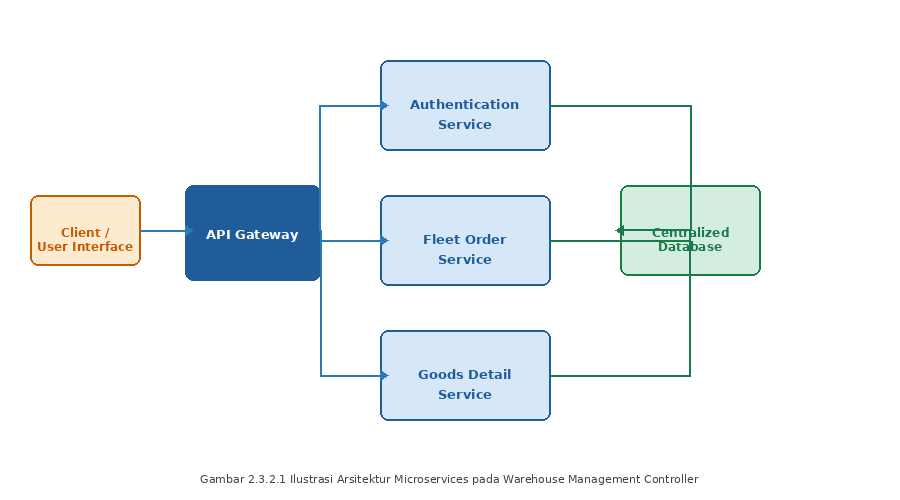
\includegraphics[width=0.85\textwidth]{images/microservices_diagram.png}
\end{figure}

\subsection{Infrastruktur Komunikasi Berbasis Message Broker}
Komunikasi antar komponen dalam sistem terdistribusi dapat dilakukan melalui dua pendekatan utama: komunikasi sinkron (\textit{request-reply} langsung seperti REST API) dan komunikasi asinkron berbasis pesan (\textit{message-passing}). Pada arsitektur WMC dan \textit{Fleet Controller} yang terdiri dari beberapa layanan independen, penggunaan mekanisme komunikasi asinkron dan \textit{real-time} menjadi kebutuhan yang tidak dapat dipenuhi oleh REST API semata. Oleh karena itu, sistem ini mengadopsi tiga infrastruktur komunikasi pelengkap, yaitu RabbitMQ sebagai \textit{message broker} antar layanan, MQTT sebagai protokol untuk komunikasi robot-server, serta WebSocket untuk pembaruan status \textit{real-time} ke \textit{User Interface}. Ketiga mekanisme ini dipilih berdasarkan evaluasi AHP yang dilakukan pada tahap analisis kebutuhan non-fungsional, khususnya untuk memenuhi KNF-02 (latensi pembaruan status $\leq$200 ms) dan KNF-06 (\textit{deployability} independen antar layanan) \autocite{docB100}.

\subsubsection{Message Broker dan RabbitMQ}
\textit{Message broker} adalah komponen perangkat lunak yang berfungsi sebagai perantara dalam pengiriman pesan antar produsen (\textit{producer}) dan konsumen (\textit{consumer}), memungkinkan kedua pihak untuk beroperasi secara asinkron dan \textit{loosely coupled} tanpa harus saling mengetahui keberadaan satu sama lain secara langsung \autocite{hohpe2003}. Pola ini pertama kali diformalkan oleh \textcite{hohpe2003} dalam \textit{Enterprise Integration Patterns} sebagai solusi integrasi sistem heterogen di mana komponen-komponen perangkat lunak berkomunikasi melalui pengiriman pesan diskrit melalui sebuah \textit{event bus} atau kanal terpusat. RabbitMQ adalah implementasi \textit{message broker} \textit{open-source} yang mengimplementasikan protokol \textit{Advanced Message Queuing Protocol} (AMQP), di mana pesan yang dipublikasikan oleh \textit{producer} dikirimkan ke \textit{exchange}, lalu diteruskan ke antrian (\textit{queue}) yang sesuai berdasarkan \textit{routing key}, dan akhirnya dikonsumsi oleh \textit{consumer} yang berlangganan pada antrian tersebut \autocite{rabbitmq2023}.

Dalam arsitektur WMC pada tugas akhir ini, RabbitMQ berperan sebagai \textit{broker} terpusat yang memfasilitasi dua jalur komunikasi utama. Pertama, komunikasi antar layanan WMC (\textit{Fleet Order Service} ke \textit{Goods Detail Service}) untuk menyampaikan \textit{event} pembaruan stok secara asinkron setelah eksekusi \textit{order}. Kedua, RabbitMQ juga bertindak sebagai MQTT \textit{broker} yang meneruskan pesan dari Subsistem Lokalisasi (\textit{Fleet Controller}) ke \textit{Fleet Order Service} melalui \textit{topic location}. Pemilihan RabbitMQ dibandingkan alternatif lain didasarkan pada kemampuannya mendukung protokol AMQP dan MQTT secara bersamaan dalam satu \textit{instance}, sehingga mengurangi jumlah komponen infrastruktur yang perlu dioperasikan secara independen, sesuai dengan prinsip KNF-06 \autocite{docB100}.

\subsubsection{Protokol MQTT untuk Komunikasi Robot-Server}
\textit{Message Queuing Telemetry Transport} (MQTT) adalah protokol komunikasi \textit{publish-subscribe} yang dirancang khusus untuk perangkat dengan keterbatasan sumber daya dan koneksi jaringan yang tidak andal, seperti perangkat IoT dan sensor terdistribusi \autocite{oasis2014}. Protokol ini bekerja dengan model tiga komponen: \textit{publisher} yang mempublikasikan pesan ke sebuah topik (\textit{topic}), \textit{broker} yang menerima dan mendistribusikan pesan, serta \textit{subscriber} yang berlangganan pada topik tertentu untuk menerima pesan secara \textit{real-time}. Keunggulan utama MQTT dibandingkan protokol komunikasi berbasis HTTP adalah \textit{overhead} yang sangat kecil---\textit{header} paket MQTT hanya berukuran minimal 2 \textit{byte}---sehingga sangat efisien untuk pengiriman data telemetri berfrekuensi tinggi seperti posisi robot yang diperbarui setiap 500 ms.

Pada sistem \textit{Smart Warehouse} ini, MQTT digunakan untuk dua jalur komunikasi yang berbeda. Pertama, Subsistem Lokalisasi mempublikasikan \textit{grid state} seluruh objek di area gudang ke \textit{topic location} setiap 500 ms. Kedua, \textit{Fleet Controller} mempublikasikan instruksi tugas (\textit{task}) ke robot melalui \textit{topic task}. \textit{Fleet Order Service} pada WMC berlangganan pada \textit{topic location} untuk meneruskan data posisi robot ke \textit{User Interface} secara \textit{real-time} melalui WebSocket, sehingga latensi \textit{end-to-end} dari pembaruan posisi fisik robot hingga tampil di layar pengguna terikat pada interval 500 ms, jauh di bawah target KNF-02 sebesar 1 detik \autocite{docB100}.

\subsubsection{WebSocket untuk Pembaruan Status Real-Time}
WebSocket adalah protokol komunikasi berbasis TCP yang memungkinkan koneksi persisten dua arah (\textit{full-duplex}) antara server dan klien, berbeda dengan paradigma \textit{request-response} pada HTTP di mana setiap pertukaran data memerlukan inisiasi koneksi baru dari sisi klien \autocite{fette2011}. Setelah koneksi WebSocket terbentuk melalui mekanisme HTTP \textit{Upgrade handshake}, server dapat mengirimkan data ke klien kapan saja tanpa harus menunggu permintaan dari klien (\textit{server push}), sehingga latensi pengiriman data hanya dibatasi oleh latensi jaringan, bukan oleh interval \textit{polling}. Keunggulan ini menjadikan WebSocket sebagai pilihan yang jauh lebih efisien dibandingkan teknik \textit{long-polling} atau \textit{Server-Sent Events} (SSE) untuk kasus penggunaan di mana data berubah secara kontinu dengan frekuensi tinggi, seperti pemantauan posisi robot secara \textit{real-time}.

Dalam implementasi WMC pada tugas akhir ini, WebSocket server diintegrasikan langsung ke dalam \textit{Fleet Order Service}. Koneksi WebSocket yang terbentuk antara server dan \textit{User Interface} menyediakan dua \textit{stream} data secara bersamaan: \textit{order stream} yang mendorong (\textit{push}) transisi status \textit{order} (\texttt{PENDING}$\rightarrow$\texttt{IN\_PROGRESS}$\rightarrow$\texttt{COMPLETED}) secara langsung tanpa \textit{polling}, serta \textit{robot stream} yang meneruskan \textit{payload} koordinat grid dan orientasi robot yang diterima dari \textit{topic} MQTT \textit{location}. Pendekatan ini memenuhi KNF-02 dengan menjamin bahwa setiap pembaruan status \textit{order} dan posisi robot dapat ditampilkan di \textit{User Interface} dalam kurun waktu yang terikat langsung pada interval publikasi Subsistem Lokalisasi (500 ms), tanpa menambah latensi dari mekanisme \textit{polling} \autocite{docB100}.

\subsection{Manajemen Basis Data Relasional untuk Inventori Real-Time}
Basis data relasional adalah sistem penyimpanan data yang mengorganisasikan informasi ke dalam tabel-tabel (relasi) yang saling terhubung melalui kunci asing (\textit{foreign key}), berdasarkan model relasional yang diperkenalkan oleh \textcite{codd1970}. Sistem ini menjamin integritas data melalui properti ACID---\textit{Atomicity}, \textit{Consistency}, \textit{Isolation}, dan \textit{Durability}---yang memastikan bahwa setiap transaksi \textit{database} dieksekusi secara penuh atau tidak sama sekali, sehingga tidak ada kondisi data yang setengah diperbarui meskipun terjadi kegagalan sistem di tengah proses \autocite{ramakrishnan2003}. Dalam konteks manajemen inventori \textit{real-time}, properti ACID menjadi sangat kritis karena setiap perubahan jumlah stok, perubahan lokasi barang, maupun pembaruan status \textit{order} harus langsung tercermin secara konsisten di seluruh layanan yang mengakses basis data secara bersamaan, tanpa risiko pembacaan data yang tidak konsisten (\textit{dirty read}) antarproses yang berjalan paralel.

Dalam arsitektur WMC pada tugas akhir ini, dipilih pendekatan basis data terpusat (\textit{centralized database}) yang menjadi satu-satunya sumber kebenaran (\textit{single source of truth}) bagi seluruh layanan \textit{microservices}. Basis data ini menyimpan empat entitas data utama, yaitu data barang (\textit{goods data}) yang mencakup identitas, jumlah, lokasi, dan kondisi stok; data pesanan (\textit{order data}) yang merekam instruksi \textit{stocking} dan \textit{picking} beserta statusnya; data sesi pengguna (\textit{session data}) untuk keperluan autentikasi; serta data sinkronisasi (\textit{synced data}) yang merepresentasikan kondisi terkini gudang untuk dikirimkan ke sistem eksternal \autocite{docB300}. Pemilihan arsitektur terpusat dibandingkan basis data terdistribusi per layanan didasarkan pada kebutuhan konsistensi yang tinggi antara \textit{Goods Detail Service}, \textit{Fleet Order Service}, dan \textit{Authentication Service}---di mana setiap \textit{query} lokasi barang oleh \textit{Fleet Order Service} harus selalu mencerminkan pembaruan terkini dari \textit{Goods Detail Service} secara langsung, tanpa mekanisme sinkronisasi tambahan yang dapat menambah latensi maupun risiko inkonsistensi data.

\section{Tinjauan Penelitian Terdahulu}

\subsection{Re-desain Proses Pemenuhan Pesanan (Framinan et al., 2025)}
\textcite{framinan2025} dalam penelitian berjudul \enquote{Redesigning the Customer Order Fulfilment Process in a Company in the FMCG Sector} yang dipublikasikan di \textit{IFAC-PapersOnLine} mengkaji proses pemenuhan pesanan pada sebuah perusahaan FMCG yang mengalami \textit{bottleneck} akibat sistem pergudangan yang masih bergantung pada proses manual. Menggunakan metode \textit{Business Process Redesign} (BPR), penelitian ini menemukan bahwa 62\% keterlambatan pengiriman bersumber dari aktivitas \textit{order picking} dan \textit{staging} yang tidak terkoordinasi secara digital, dan menegaskan bahwa sistem \textit{warehouse} konvensional tidak mampu memenuhi tuntutan permintaan tinggi dan variasi SKU yang luas tanpa dukungan teknologi otomasi dan integrasi sistem informasi yang menyeluruh. Temuan ini memiliki relevansi langsung terhadap kondisi operasional gudang barang jadi Paragon Corp, di mana ketergantungan pada operator dalam proses \textit{stocking} dan \textit{picking}---serta ketiadaan integrasi \textit{real-time} antara WMS lokal dengan sistem pusat---menghasilkan pola inefisiensi yang paralel: \textit{lead time} yang panjang, \textit{mismatch} data inventori, dan tingginya risiko \textit{human error}. Penelitian ini memperkuat urgensi pengembangan WMC sebagai solusi digitalisasi yang secara langsung merespons akar permasalahan yang diidentifikasi oleh \textcite{framinan2025}.

\subsection{Integrasi Cloud dan IoT untuk Visibilitas Gudang (van Geest et al., 2021)}
\textcite{vangeest2021} dalam artikel ilmiah berjudul \enquote{Smart Warehouses: Rationale, Challenges, and Solution Directions} yang diterbitkan di jurnal \textit{Computers in Industry} menyajikan \textit{systematic review} mengenai evolusi \textit{Smart Warehouse} sebagai respons terhadap meningkatnya kompleksitas rantai pasok modern. Penelitian ini mengidentifikasi empat pilar \textit{technology enabler} utama \textit{Smart Warehouse}, yaitu \textit{Automation and Robotics} (penggunaan AGV/AMR untuk transportasi internal), \textit{IoT-based Visibility} (sensor dan RFID untuk deteksi posisi barang secara \textit{real-time}), \textit{AI-driven Optimization} (penjadwalan dan penentuan rute otomatis), serta \textit{Cyber-Physical Integration} sebagai sinergi antara operasi fisik dan sistem digital berbasis \textit{cloud}. Selain mengidentifikasi pilar-pilar tersebut, penulis juga mengklasifikasikan tantangan implementasi ke dalam tiga kategori, yaitu tantangan operasional (integrasi multi-robot dan koordinasi sistem), tantangan teknologi (interoperabilitas antar platform, latensi \textit{cloud}, dan keamanan siber), serta tantangan organisasi (resistensi sumber daya manusia dan biaya transformasi). Relevansi penelitian ini terhadap tugas akhir sangat substansial: kondisi Paragon Corp yang masih berada pada tahap awal integrasi digital secara langsung mencerminkan tantangan teknologi yang diidentifikasi \textcite{vangeest2021}, sementara arsitektur WMC yang dikembangkan---dengan basis data terpusat dan pencatatan \textit{event real-time}---merupakan implementasi konkret dari pilar \textit{Cyber-Physical Integration} yang direkomendasikan penelitian tersebut untuk meningkatkan konsistensi distribusi dan visibilitas stok secara menyeluruh.

\subsection{Implementasi Event-Driven Architecture pada Sistem Manajemen Inventori Real-Time}
\textcite{hohpe2003} dalam \textit{Enterprise Integration Patterns} meletakkan fondasi teoritis arsitektur berbasis \textit{event} sebagai paradigma integrasi sistem di mana komponen-komponen perangkat lunak berkomunikasi melalui pengiriman dan penerimaan pesan (\textit{event}) secara asinkron melalui sebuah \textit{event bus} atau \textit{broker} terpusat, sehingga setiap komponen tetap \textit{loosely coupled} dan dapat beroperasi secara independen tanpa harus mengetahui keberadaan komponen lain secara langsung. Dalam konteks manajemen inventori \textit{real-time}, pendekatan ini diwujudkan melalui tiga kategori komponen utama: \textit{event producers} yang menghasilkan \textit{event} (seperti \textit{Fleet Controller}, \textit{Order System}, dan \textit{User Interface}), \textit{event bus} sebagai kanal distribusi pesan, serta \textit{event consumers} yang memproses \textit{event} sesuai tanggung jawabnya masing-masing (seperti \textit{Inventory Update Handler}, \textit{Order Status Handler}, dan \textit{Notification Handler}), sebagaimana diilustrasikan pada Gambar \ref{fig:eda-diagram}. Setiap perubahan kondisi inventori---mulai dari eksekusi tugas robot, pembaruan status pesanan, hingga konfirmasi pengiriman barang---dipublikasikan sebagai \textit{event} diskrit yang kemudian dikonsumsi oleh \textit{handler} terkait untuk memperbarui \textit{state} pada basis data terpusat secara atomik \autocite{docB300}. Relevansi tinjauan ini terhadap tugas akhir terletak pada adopsi pola yang sama dalam arsitektur WMC: \textit{Order Status Event}, \textit{Robot Task Event}, dan \textit{Robot Status Event} masing-masing diproses oleh \textit{handler} yang berbeda di dalam layanan \textit{Fleet Order Service} dan \textit{Goods Detail Service}, menjamin bahwa data inventori di basis data terpusat selalu mencerminkan kondisi fisik terkini di lapangan tanpa ketergantungan langsung antar layanan.

\begin{figure}[t]
  \caption{Ilustrasi alur \textit{Event-Driven Architecture} pada sistem manajemen inventori}
  \label{fig:eda-diagram}
  \centering
  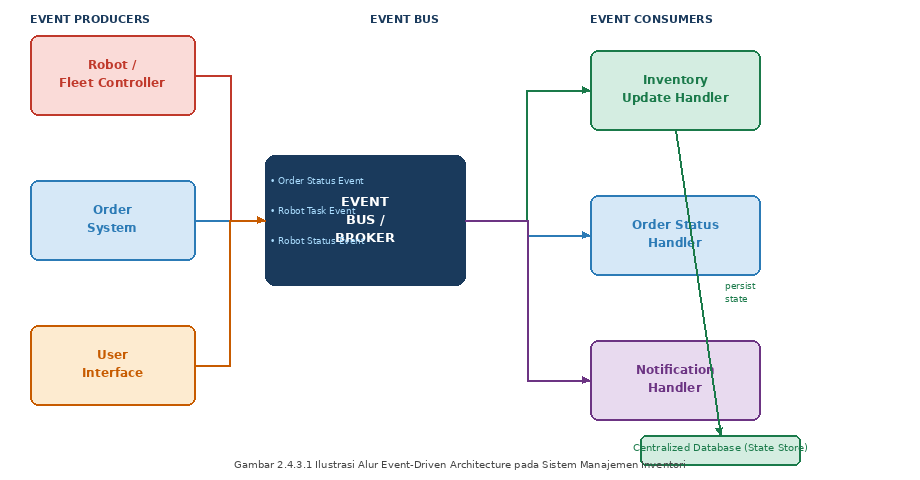
\includegraphics[width=0.85\textwidth]{images/eda_diagram.png}
\end{figure}

\section{Landasan Teori: Subsistem Lokalisasi}

\subsection{AprilTag sebagai Fiducial Marker}
AprilTag adalah sistem \textit{fiducial marker} yang dikembangkan untuk keperluan \textit{computer vision} pada aplikasi robotika. Setiap \textit{tag} mengodekan ID unik dalam format pola biner berdasarkan keluarga kode tertentu, sehingga detektor dapat membedakan ratusan \textit{tag} secara bersamaan dalam satu \textit{frame} kamera. Keunggulan utama AprilTag dibandingkan alternatif seperti QR Code atau ArUco adalah kemampuannya memberikan estimasi \textit{pose} 6-DOF (\textit{degree of freedom}) secara lengkap---mencakup posisi (X, Y, Z) dan orientasi (\textit{roll}, \textit{pitch}, \textit{yaw})---dari satu gambar kamera \textit{monocular} tanpa infrastruktur \textit{sensing} aktif \autocite{hartley2004}. Dalam proyek ini, digunakan keluarga Tag36h11 berukuran fisik 8$\times$8 cm yang ditempelkan pada robot dan barang di lantai gudang untuk keperluan identifikasi serta penentuan posisi dan orientasi secara \textit{overhead}. Konfigurasi kamera \textit{overhead} dipilih karena memungkinkan satu kamera yang dipasang di langit-langit untuk mengamati seluruh area lantai gudang tanpa oklusi dari rak atau robot \autocite{bradski2000}.

\subsection{Koreksi Distorsi Lensa Fisheye (Model Kannala--Brandt)}
Lensa \textit{fisheye} menyediakan sudut pandang yang sangat lebar sehingga memungkinkan satu kamera yang dipasang di langit-langit untuk mengamati seluruh area lantai gudang dari satu titik pemasangan. Namun, optik \textit{fisheye} memperkenalkan distorsi radial yang parah: garis lurus tampak melengkung pada gambar dan jarak piksel tidak seragam di seluruh \textit{frame}, sehingga pemetaan langsung dari koordinat piksel ke posisi fisik menjadi tidak valid \autocite{bradski2000}. Distorsi ini harus dikoreksi sebelum operasi geometri apa pun dapat dilakukan pada gambar.

Model kalibrasi Kannala--Brandt merupakan model polinomial berbasis proyeksi ekuidistansi yang memodelkan distorsi lensa \textit{fisheye} melalui serangkaian koefisien kalibrasi. Koefisien ini dihitung saat proses \textit{setup} kalibrasi menggunakan pola papan catur (\textit{checkerboard}) yang diletakkan di berbagai sudut dan jarak di depan kamera. Setelah koefisien diperoleh, proses \textit{undistortion} diterapkan pada setiap \textit{frame} video menggunakan OpenCV sebelum pemrosesan lebih lanjut, menghasilkan gambar yang secara geometri konsisten dan valid untuk operasi perspektif selanjutnya.

\subsection{Perspective Homography dan Pemetaan Koordinat Grid}
Setelah koreksi distorsi lensa, koordinat piksel dari titik tengah \textit{tag} yang terdeteksi perlu diubah menjadi koordinat posisi di lantai gudang. Transformasi ini dilakukan menggunakan \textit{perspective homography}, yaitu transformasi projektif yang memetakan titik pada satu bidang datar ke bidang datar lainnya. \textit{Homography} merupakan transformasi yang tepat untuk kasus ini karena lantai gudang bersifat planar dan kamera mengamatinya dari atas secara tegak lurus, sehingga setiap titik di lantai memiliki korespondensi satu-ke-satu dengan piksel di citra \autocite{hartley2004}.

Secara matematis, \textit{perspective homography} direpresentasikan sebagai matriks $H$ berukuran $3\times3$. Representasi ini menggunakan koordinat homogen, yaitu skema di mana titik 2D $(u, v)$ diangkat ke ruang tiga dimensi sebagai triplet $(u, v, 1)$. Dimensi ketiga ini memungkinkan transformasi perspektif---yang secara inheren non-linear akibat adanya pembagian---ditulis ulang dalam bentuk perkalian matriks linear \autocite{bradski2000}. Perkalian matriks menghasilkan triplet antara $(g'_x, g'_y, w')$ yang kemudian dikembalikan ke koordinat 2D melalui \textit{perspective division}, yaitu pembagian dengan komponen ketiga $w'$:
\begin{equation}
(g'_x, g'_y, w') = H \cdot (u, v, 1)
\label{eq:homography}
\end{equation}
dengan
\begin{equation}
H = \begin{bmatrix} h_{00} & h_{01} & h_{02} \\ h_{10} & h_{11} & h_{12} \\ h_{20} & h_{21} & 1 \end{bmatrix}
\label{eq:homography-matrix}
\end{equation}

Elemen ke-9 matriks $H$ dinormalisasi menjadi $h_{22} = 1$ sehingga $H$ memiliki 8 derajat kebebasan. Koordinat lantai kontinu $(g_x, g_y)$ diperoleh melalui \textit{perspective division} terhadap hasil perkalian matriks tersebut:
\begin{align}
g_x &= \frac{h_{00} \cdot u + h_{01} \cdot v + h_{02}}{h_{20} \cdot u + h_{21} \cdot v + 1} \label{eq:gx}\\
g_y &= \frac{h_{10} \cdot u + h_{11} \cdot v + h_{12}}{h_{20} \cdot u + h_{21} \cdot v + 1} \label{eq:gy}
\end{align}

Matriks $H$ dihitung satu kali pada tahap kalibrasi dari empat titik korespondensi yang diketahui: empat sudut area lantai gudang yang koordinat pikselnya $(u_i, v_i)$ diperoleh melalui klik manual pengguna pada citra kalibrasi, dan koordinat \textit{grid} targetnya $(g_{xi}, g_{yi})$ ditetapkan sebagai sudut-sudut \textit{rectangle grid}, yaitu $(0,0)$, $(C,0)$, $(C,R)$, dan $(0,R)$ dengan $C = 8$ kolom dan $R = 4$ baris. Setiap pasangan korespondensi menghasilkan dua persamaan linear setelah perkalian silang menghilangkan penyebut \autocite{hartley2004}:
\begin{align}
h_{00} u_i + h_{01} v_i + h_{02} - h_{20} u_i g_{xi} - h_{21} v_i g_{xi} &= g_{xi} \label{eq:linear1}\\
h_{10} u_i + h_{11} v_i + h_{12} - h_{20} u_i g_{yi} - h_{21} v_i g_{yi} &= g_{yi} \label{eq:linear2}
\end{align}

Dengan empat titik korespondensi, terbentuk sistem linear $8\times8$ dalam vektor parameter $h = (h_{00}, h_{01}, h_{02}, h_{10}, h_{11}, h_{12}, h_{20}, h_{21})$ yang diselesaikan secara eksak karena jumlah persamaan sama dengan jumlah variabel. Penyelesaian sistem linear ini dilakukan secara internal oleh fungsi \texttt{getPerspectiveTransform} pada pustaka OpenCV, sehingga pengguna hanya perlu menyediakan empat pasang titik korespondensi untuk memperoleh matriks $H$ yang lengkap \autocite{bradski2000}.

Koordinat lantai kontinu $(g_x, g_y)$ yang diperoleh kemudian di-\textit{snap} ke sel \textit{grid} diskrit $(c, r)$ menggunakan aturan \textit{nearest-cell-centre}. Karena setiap sel berukuran $1\times1$ dalam satuan \textit{grid} dan berpusat pada titik $(c + 0,5, r + 0,5)$, formula \textit{snap} adalah:
\begin{align}
c &= \text{clip}(\text{round}(g_x - 0,5), 0, 7) \label{eq:snap-c}\\
r &= \text{clip}(\text{round}(g_y - 0,5), 0, 3) \label{eq:snap-r}
\end{align}

Operasi \textit{clip} memastikan indeks sel tidak keluar dari batas \textit{grid} $8\times4$, sehingga seluruh titik di area lantai gudang ($2,4 \times 1,2$ m) selalu terpetakan ke dalam 32 sel yang valid. Pendekatan ini memungkinkan satu kamera \textit{overhead} memetakan posisi seluruh robot, barang, dan \textit{docking station} ke representasi \textit{grid} diskrit secara \textit{real-time} tanpa sensor tambahan.
